\documentclass[]{article}
\usepackage{lmodern}
\usepackage{amssymb,amsmath}
\usepackage{ifxetex,ifluatex}
\usepackage{fixltx2e} % provides \textsubscript
\ifnum 0\ifxetex 1\fi\ifluatex 1\fi=0 % if pdftex
  \usepackage[T1]{fontenc}
  \usepackage[utf8]{inputenc}
\else % if luatex or xelatex
  \ifxetex
    \usepackage{mathspec}
  \else
    \usepackage{fontspec}
  \fi
  \defaultfontfeatures{Ligatures=TeX,Scale=MatchLowercase}
\fi
% use upquote if available, for straight quotes in verbatim environments
\IfFileExists{upquote.sty}{\usepackage{upquote}}{}
% use microtype if available
\IfFileExists{microtype.sty}{%
\usepackage{microtype}
\UseMicrotypeSet[protrusion]{basicmath} % disable protrusion for tt fonts
}{}
\usepackage[margin=1in]{geometry}
\usepackage{hyperref}
\hypersetup{unicode=true,
            pdftitle={Project1},
            pdfborder={0 0 0},
            breaklinks=true}
\urlstyle{same}  % don't use monospace font for urls
\usepackage{color}
\usepackage{fancyvrb}
\newcommand{\VerbBar}{|}
\newcommand{\VERB}{\Verb[commandchars=\\\{\}]}
\DefineVerbatimEnvironment{Highlighting}{Verbatim}{commandchars=\\\{\}}
% Add ',fontsize=\small' for more characters per line
\usepackage{framed}
\definecolor{shadecolor}{RGB}{248,248,248}
\newenvironment{Shaded}{\begin{snugshade}}{\end{snugshade}}
\newcommand{\KeywordTok}[1]{\textcolor[rgb]{0.13,0.29,0.53}{\textbf{#1}}}
\newcommand{\DataTypeTok}[1]{\textcolor[rgb]{0.13,0.29,0.53}{#1}}
\newcommand{\DecValTok}[1]{\textcolor[rgb]{0.00,0.00,0.81}{#1}}
\newcommand{\BaseNTok}[1]{\textcolor[rgb]{0.00,0.00,0.81}{#1}}
\newcommand{\FloatTok}[1]{\textcolor[rgb]{0.00,0.00,0.81}{#1}}
\newcommand{\ConstantTok}[1]{\textcolor[rgb]{0.00,0.00,0.00}{#1}}
\newcommand{\CharTok}[1]{\textcolor[rgb]{0.31,0.60,0.02}{#1}}
\newcommand{\SpecialCharTok}[1]{\textcolor[rgb]{0.00,0.00,0.00}{#1}}
\newcommand{\StringTok}[1]{\textcolor[rgb]{0.31,0.60,0.02}{#1}}
\newcommand{\VerbatimStringTok}[1]{\textcolor[rgb]{0.31,0.60,0.02}{#1}}
\newcommand{\SpecialStringTok}[1]{\textcolor[rgb]{0.31,0.60,0.02}{#1}}
\newcommand{\ImportTok}[1]{#1}
\newcommand{\CommentTok}[1]{\textcolor[rgb]{0.56,0.35,0.01}{\textit{#1}}}
\newcommand{\DocumentationTok}[1]{\textcolor[rgb]{0.56,0.35,0.01}{\textbf{\textit{#1}}}}
\newcommand{\AnnotationTok}[1]{\textcolor[rgb]{0.56,0.35,0.01}{\textbf{\textit{#1}}}}
\newcommand{\CommentVarTok}[1]{\textcolor[rgb]{0.56,0.35,0.01}{\textbf{\textit{#1}}}}
\newcommand{\OtherTok}[1]{\textcolor[rgb]{0.56,0.35,0.01}{#1}}
\newcommand{\FunctionTok}[1]{\textcolor[rgb]{0.00,0.00,0.00}{#1}}
\newcommand{\VariableTok}[1]{\textcolor[rgb]{0.00,0.00,0.00}{#1}}
\newcommand{\ControlFlowTok}[1]{\textcolor[rgb]{0.13,0.29,0.53}{\textbf{#1}}}
\newcommand{\OperatorTok}[1]{\textcolor[rgb]{0.81,0.36,0.00}{\textbf{#1}}}
\newcommand{\BuiltInTok}[1]{#1}
\newcommand{\ExtensionTok}[1]{#1}
\newcommand{\PreprocessorTok}[1]{\textcolor[rgb]{0.56,0.35,0.01}{\textit{#1}}}
\newcommand{\AttributeTok}[1]{\textcolor[rgb]{0.77,0.63,0.00}{#1}}
\newcommand{\RegionMarkerTok}[1]{#1}
\newcommand{\InformationTok}[1]{\textcolor[rgb]{0.56,0.35,0.01}{\textbf{\textit{#1}}}}
\newcommand{\WarningTok}[1]{\textcolor[rgb]{0.56,0.35,0.01}{\textbf{\textit{#1}}}}
\newcommand{\AlertTok}[1]{\textcolor[rgb]{0.94,0.16,0.16}{#1}}
\newcommand{\ErrorTok}[1]{\textcolor[rgb]{0.64,0.00,0.00}{\textbf{#1}}}
\newcommand{\NormalTok}[1]{#1}
\usepackage{graphicx,grffile}
\makeatletter
\def\maxwidth{\ifdim\Gin@nat@width>\linewidth\linewidth\else\Gin@nat@width\fi}
\def\maxheight{\ifdim\Gin@nat@height>\textheight\textheight\else\Gin@nat@height\fi}
\makeatother
% Scale images if necessary, so that they will not overflow the page
% margins by default, and it is still possible to overwrite the defaults
% using explicit options in \includegraphics[width, height, ...]{}
\setkeys{Gin}{width=\maxwidth,height=\maxheight,keepaspectratio}
\IfFileExists{parskip.sty}{%
\usepackage{parskip}
}{% else
\setlength{\parindent}{0pt}
\setlength{\parskip}{6pt plus 2pt minus 1pt}
}
\setlength{\emergencystretch}{3em}  % prevent overfull lines
\providecommand{\tightlist}{%
  \setlength{\itemsep}{0pt}\setlength{\parskip}{0pt}}
\setcounter{secnumdepth}{0}
% Redefines (sub)paragraphs to behave more like sections
\ifx\paragraph\undefined\else
\let\oldparagraph\paragraph
\renewcommand{\paragraph}[1]{\oldparagraph{#1}\mbox{}}
\fi
\ifx\subparagraph\undefined\else
\let\oldsubparagraph\subparagraph
\renewcommand{\subparagraph}[1]{\oldsubparagraph{#1}\mbox{}}
\fi

%%% Use protect on footnotes to avoid problems with footnotes in titles
\let\rmarkdownfootnote\footnote%
\def\footnote{\protect\rmarkdownfootnote}

%%% Change title format to be more compact
\usepackage{titling}

% Create subtitle command for use in maketitle
\newcommand{\subtitle}[1]{
  \posttitle{
    \begin{center}\large#1\end{center}
    }
}

\setlength{\droptitle}{-2em}

  \title{Project1}
    \pretitle{\vspace{\droptitle}\centering\huge}
  \posttitle{\par}
    \author{}
    \preauthor{}\postauthor{}
    \date{}
    \predate{}\postdate{}
  
\usepackage{amsmath}

\begin{document}
\maketitle

\newcommand{\vect}[1]{\boldsymbol{\mathbf{#1}}}
\newcommand{\matr}[1]{\boldsymbol{\mathbf{#1}}}
\newcommand{\det}{det}
\newcommand{\exp}{exp}
\newcommand{\exp}{iid}

\[E(r(X)) = \mu_r = 0\]

\[Var(r(X)) = \sigma_r^2\] \[ Cor(r(X), r(X')) = \rho_r(\tau) \]

\[\tau = \frac{| X - X'|}{10}\]

\((r(x) | x\in D = [1, 50]\subset \mathbb{R}^1)\)

\(\vect{X}\)

\begin{Shaded}
\begin{Highlighting}[]
\NormalTok{p1}
\end{Highlighting}
\end{Shaded}

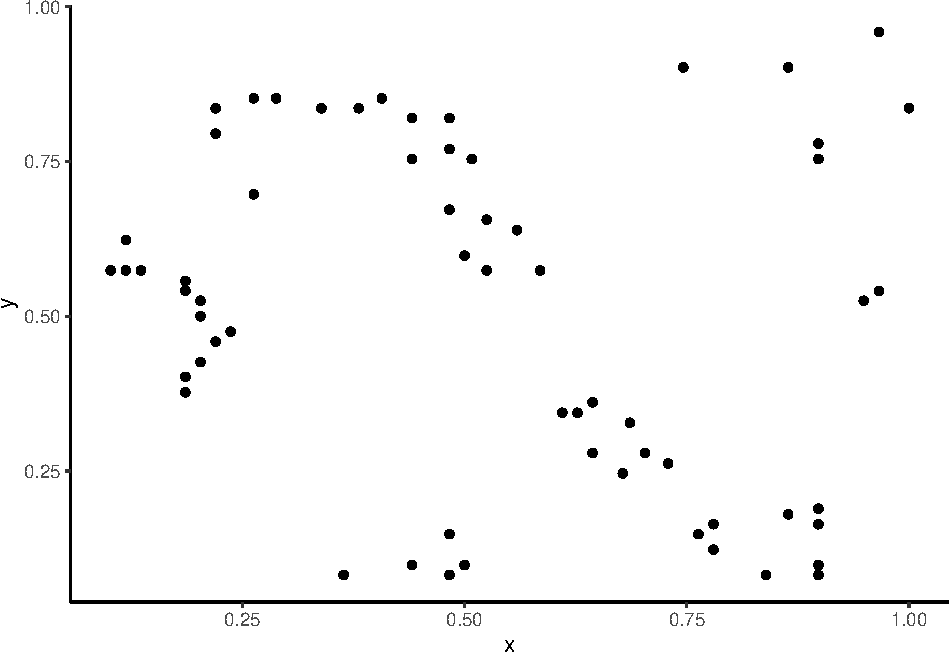
\includegraphics{Project1_files/figure-latex/unnamed-chunk-1-1.pdf}

\begin{Shaded}
\begin{Highlighting}[]
\NormalTok{p2}
\end{Highlighting}
\end{Shaded}

\begin{verbatim}
## $x
##   [1] 0.00 0.02 0.04 0.06 0.08 0.10 0.12 0.14 0.16 0.18 0.20 0.22 0.24 0.26
##  [15] 0.28 0.30 0.32 0.34 0.36 0.38 0.40 0.42 0.44 0.46 0.48 0.50 0.52 0.54
##  [29] 0.56 0.58 0.60 0.62 0.64 0.66 0.68 0.70 0.72 0.74 0.76 0.78 0.80 0.82
##  [43] 0.84 0.86 0.88 0.90 0.92 0.94 0.96 0.98 1.00 1.02 1.04 1.06 1.08 1.10
##  [57] 1.12 1.14 1.16 1.18 1.20 1.22 1.24 1.26 1.28 1.30 1.32 1.34 1.36 1.38
##  [71] 1.40 1.42 1.44 1.46 1.48 1.50 1.52 1.54 1.56 1.58 1.60 1.62 1.64 1.66
##  [85] 1.68 1.70 1.72 1.74 1.76 1.78 1.80 1.82 1.84 1.86 1.88 1.90 1.92 1.94
##  [99] 1.96 1.98 2.00
## 
## $y
##   [1] 0.000000000 0.002480177 0.009751414 0.021441687 0.037095899
##   [6] 0.056227056 0.078345060 0.102974160 0.129663619 0.157994004
##  [11] 0.187580551 0.218074523 0.249163212 0.280568995 0.312047777
##  [16] 0.343387041 0.374403659 0.404941590 0.434869552 0.464078717
##  [21] 0.492480491 0.520004387 0.546596024 0.572215256 0.596834443
##  [26] 0.620436855 0.643015218 0.664570386 0.685110151 0.704648156
##  [31] 0.723202937 0.740797058 0.757456347 0.773209225 0.788086105
##  [36] 0.802118880 0.815340463 0.827784403 0.839484543 0.850474735
##  [41] 0.860788596 0.870459301 0.879519418 0.888000763 0.895934294
##  [46] 0.903350018 0.910276925 0.916742937 0.922774875 0.928398442
##  [51] 0.933638204 0.938517600 0.943058948 0.947283457 0.951211254
##  [56] 0.954861403 0.958251944 0.961399914 0.964321392 0.967031528
##  [61] 0.969544584 0.971873971 0.974032286 0.976031353 0.977882255
##  [66] 0.979595378 0.981180442 0.982646539 0.984002166 0.985255260
##  [71] 0.986413227 0.987482977 0.988470949 0.989383142 0.990225143
##  [76] 0.991002149 0.991718994 0.992380172 0.992989858 0.993551928
##  [81] 0.994069984 0.994547363 0.994987164 0.995392257 0.995765303
##  [86] 0.996108769 0.996424935 0.996715916 0.996983666 0.997229995
##  [91] 0.997456574 0.997664950 0.997856552 0.998032700 0.998194614
##  [96] 0.998343419 0.998480155 0.998605780 0.998721181 0.998827173
## [101] 0.998924509
\end{verbatim}

\# Problem 1b) Want to specify pdf of a guassian prior rf.

Let
\(\vect r \sim p(\vect r) = \phi_n(\vect r | \mu_r\vect 1_n, \sigma^2_r \matr \Sigma_r^\rho\)
With \(\matr \Sigma_r^p\) covariance matrix defined by the corrolation
function given in problem 1a) for a given \(\kappa\). To start off we
select \(\kappa = 0.5\).

This would give use the following pdf:
\[f_{\vect r}(\vect r | \mu_r, \sigma_r^2\matr \Sigma_r^\rho)= (2\pi)^{-\frac{n}{2}}det(\matr\Sigma_r^\rho)^{-\frac{1}{2}}\exp\left(-\frac{1}{2}\left(\vect r - \mu_r\vect 1_n\right)^T(\matr\Sigma_r^\rho)^{-1}\left(\vect r - \mu_r\vect 1_n\right)\right)\]

\section{Problem 1c)}\label{problem-1c}

\begin{equation*}
   d(x) = r(x) + \epsilon(x), \quad x \in \lbrace 10, 25, 30 \rbrace \\
   \epsilon(\dot) \sim N(0, \sigma_\epsilon^2), \iid \\
   d(x) \sim aquistion model \\
   r(x) and \epsilon(x) indep \\
   \epsilon(x) and \epsilon(x') \iid  \\
\end{equation*}

As we both \(\epsilon(\dot)\) and \(r(\dot)\) ar gaussian, a linear
product of the two would also be.

We further note: \[E(d(x)) = E(r(x)) + E((\epsilon(x))) = 0\]

When \(x\neq x'\)
\[Cov(d(x), d(x')) = Cov(r(x)+\epsilon(x), r(x') + \epsilon(x')) = Cov(r(x), r(x')) + Cov(\epsilon(x), \epsilon(x')) = \sigma_r^2\rho_r(\tau)\]
And:
\[Cov(d(x), d(x)) = Cov(r(x)+\epsilon(x), r(x) + \epsilon(x)) = Cov(r(x), r(x)) + Cov(\epsilon(x), \epsilon(x)) = \sigma_r^2\rho_r(\tau) + \sigma_e^2\]

So in general we see:
\[Cov(\vect d(\vect x), \vect d(\vect x')) = \sigma^2_e \matr I_k +\sigma^2_r\matr \Sigma_\rho^d\]

\(\vect d\) is multivariate normal and thus have the following pdf:
\[p(\vect d(\vect x)|\sigma_r^2, \sigma_e^2) = (2\pi)^{k/2}det(\matr \Sigma_\rho^d)^{-1/2}\exp(\frac{1}{2}\vect d^T(\matr\Sigma_\rho^d)^{-1}\vect d)\]

With the corresponding likelihood function:
\[L(\sigma_e^2 | \vect d(\vect x), \sigma_r^2)=p(\vect d(\vect x)|\sigma_r^2, \sigma_e^2)\]
The integral
\[\int_{0}^{\infty}p(\vect d(\vect x)|\sigma_r^2, \sigma_e^2) d\sigma^2\]
goes to infinity, thus not a pdf. If we try to draw sigmas beliving L is
a pdf, we would expect values to goes to infinity, which would give us
more variance than we have.

\section{Problem 1d)}\label{problem-1d}

\(\vect d(\vect x)\) and \(\vect l(\vect x)\) are both multivariate
gaussian so \(\vect l | \vect d\) would also be. Have:

\[
  \vect\mu_{\vect l | \vect d} = \vect \mu_l + \matr \Sigma_{\vect l, \vect d}^\rho \matr \Sigma_{\vect d, \vect d}^{-1}(\vect d - \vect \mu_{\vect d})
\]

\[
  \vect\Sigma_{\vect l | \vect d}^\rho = \matr \Sigma_{\vect l}^\rho - \matr \Sigma_{\vect l, \vect d}^\rho \matr \Sigma_{\vect d, \vect d}^{-1}\Sigma_{\vect d, \vect l}^\rho
\]


\end{document}
